\section{Motivation}
\label{sec:motivation}
In der Quantenmechanik sind Experimente und Messungen schwierig, aufgrund der Systemgrößen
und der Entkopplung von Umgebung und System.
In diesem Versuch werden drei Systeme betrachtet, deren quantenmeschanische Eigenschaften mit Phänomenen der klassischen und analytischen Mechanik verglichen werden können, insbesondere unter dem Gesichtspunkt von Resonanzen.
\section{Theorie}
\label{sec:Theorie}
\subsection{Zylinderresonator}
In einem Zylinder entstehen Resonanzen, wenn die reflekierten Wellen konstruktiv miteinander interferieren.
Die Resonanzfrequenz eines geschlossenen Zylinders folgt aus der Bedingung das der Druck an den Enden maximal ist.
Zur Beschreibung startet man mit der \glname{Helmholtz}{gleichung}
\begin{align}
    \partial_t^2p(\vec{r},t) &= \frac{1}{ρκ}\laplace p(\vec{r},t)\\
    ρ &: \text{Dichte}\\
    κ &: \text{Kompressibilität}
    \shortintertext{und dem Ansatz}
    p(\vec{r},t) &= p(\vec{r})\cdot\cos(ωt)\:.
    \intertext{Dieser genügt den oben genannten Randbedingungen und liefert}
    p(\vec{r}) &= -\frac{1}{ω^2ρκ}\laplace p(\vec{r})\:.
    \intertext{Daraus, und Abbildung \ref{fig:schwingung} ergibt sich die Wellenlänge zu}
    λ_N &= \frac{2L}{N} \label{eqn:resonanzlaenge}
    \intertext{mit der Länge $L$ des Zylinders und $N$ als Ordnung der Resonanz. Mit der Schallgeschwindigkeit}
    c &= λf
    \shortintertext{ergibt sich die Frequenz zu}
    f_N &= \frac{cN}{2L}\:. \label{eqn:resonanzfrequenz}
\end{align}

\begin{figure}
    \centering
    \includegraphics[width=0.4\textwidth]{build/theorie-schwingung.pdf}
    \caption{Grund- \& 1. Oberschwingung in einem geschlossenen Zylinder.\\
              Aufgetragen ist die Druckamplitude gegen die Position im Zylinder.}
    \label{fig:schwingung}
\end{figure}

Abbildung \ref{fig:schwingung} zeigt die Grundschwingung und die erste Oberschwingung, in der Quantenmechanik kann dieses System mit einem Teilchen in einem Kastenpotential wiedergefunden werden.
Für dieses System gilt die \glname{Schrödinger}{-Gleichung} in der Form
\begin{align}
  i\hbar\partial_tψ(x,t) &= -\frac{\hbar^2}{2m}\laplaceψ(x,t)+V(x)ψ(x,t)
  \shortintertext{mit dem Potential}
  V(x) &= \begin{cases}0,\quad0\leq x\leq\text{L}\\\infty,\qquad\text{sonst}\end{cases}
  \shortintertext{Der Separationsansatz}
  ψ(x,t) &= ψ(x)\me^{iωt}
  \intertext{vereinfacht die \glname{Schrödinger}{-Gleichung} auf}
  \hbarωψ(x) &= \frac{\hbar^2}{2m}\partial_x^2ψ(x)\:.
  \intertext{Hierfür ist die Lösung}
  ψ(x) &= A\sin({k_nx})
  \shortintertext{mit}
  k_n &= \mpi\frac{n}{\symup{L}} = \sqrt{\frac{2mω}{\hbar}}
  \intertext{bekannt, und passt mit}
  k &= \frac{2\mpi}{λ}
  \intertext{zur Bedingung \eqref{eqn:resonanzlaenge} der klassischen Betrachtung:}
  \frac{1}{λ} &= \frac{N}{2L}\:.
\end{align}

\subsection{Kugelresonator}
Die Betrachtung des Kugelresonators zieht eine Koordinatentransformation mit sich.
Im Experiment wird nur der Winkel $α$ gemessen. Der Separationsansatz
\begin{align}
  p(\vec{r}) &= p(r)Y_{lm}(θ,φ)
  \intertext{mit den Kugelflächenfunktionen und Argumenten $θ\:\&\:φ$ zieht eine Transformation nach. Die Beziehung}
  φ &= α
  \intertext{wird ersichtlich wenn die Kugelhälften um einen beliebigen Winkel verdreht werden.
    Für die Bestimmung von $θ$ legt man zunächst die Positon des Lautsprechers auf}
  \vec{r}_L &= r\begin{pmatrix}\frac{1}{\sqrt{2}}\\0\\-\frac{1}{\sqrt{2}}\\\end{pmatrix}
  \intertext{fest. Das Mikrofon beschreibt einen Kreis auf einer festen Höhe von}
  z &= \frac{1}{\sqrt{2}}
  \intertext{damit folgt für die Position}
  \vec{r}_M &= r
  \begin{pmatrix}\frac{\cos(α)}{\sqrt{2}}\\\frac{\sin(α)}{\sqrt{2}}\\\frac{1}{\sqrt{2}}\\\end{pmatrix}
    \intertext{$θ$ ist der Winkel zwischen diesen beiden Vektoren und somit}
    \cos(θ) &= \frac{\vec{r}_M\cdot\vec{r}_L}{\abs{\vec{r}_M}\cdot\abs{\vec{r}_L}}
    = \frac{1}{2}(\cos(α)-1)\:. \label{eqn:costheta}
\end{align}

\subsection{Wasserstoffatom}
Die zeitunabhängige \glname{Schrödinger}{-Gleichung} des Wasserstoffatoms lautet
\begin{equation}
  Eψ(\vec{r}) = -\frac{\hbar^2}{2m}\laplaceψ(\vec{r})+V(\vec{r})ψ(\vec{r})\:.
\end{equation}
Aufgrund der Symmetrie des Systems ist der Laplaceoperator in Kugelkoordinaten zu wählen,
dadurch kann auch hier die Lösung mittels einer Separation ermittelt werden.
Der winkelabängige Teil der Gleichung wird wieder von den Kugelfächenfunktionen gelöst.

\subsection{Wasserstoffmolekül}
Auch das Wasserstoffmolekül wird durch eine \glname{Schrödinger}{-Gleichung}
beschrieben, diese hat nun zwei Lösungen.
Da beim Überlapp der Orbitale vom $H^+_2$ Molekül eine Phasenverschiebung
von $\pi$ vorkommen kann und diese auch ein vernünftiges Ergebnis liefert.
Abhängig vom Vorzeichen gibt es nun bindende- und antibindende Orbitale.
Bei antibindenden Orbitalen verschwindet die Aufenthaltswahrscheinlichkeit
für die Elektronen zwischen den Atomkernen. In Abb. \ref{fig:orbital} ist
eine schematische Abbildung dieser Orbitale zusehen, genommen aus \cite{orbitale}.
\begin{figure}
  \centering
    \caption{Bindende und Antibindende Orbitale in Ethen.}
    \label{fig:orbital}
    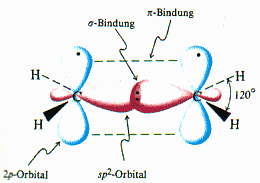
\includegraphics[width=0.5\textwidth]{pdfs/orbital.png}
\end{figure}

Eine exakte Beschreibung dieser Orbitale liegt der magnetischen Quantenzahl m
zugrunde. Bei der Überlagerung von zwei Orbitalen mit $m = 0$, spricht man
von einem $\sigma$-Orbital. Bei zwei $|m| = 1$ Orbitalen hingegen von $\pi$
Orbitalen.
\\
Mit der Hauptquantenzahl werden hier auch Elektronen unterschiedlicher
Energie im selben Orbital unterschieden, wobei wir hier die $1\sigma_y$ und
die 1s Zustände nicht untersuchen können, da diesen eine konstante
Druckverteilung im Resonator entspricht und diesem eine Resonanzfrequenz von 0
Hz entspricht.
\\
Bei der Überlagerung von zwei Orbitalen mit Hauptquantenzahl $n = 2$
entstehen zum einen $σ$- als auch $π$-Orbitale. Auch dort gibt es wieder
bindende- und antibindende-Orbitale.

\subsection{1-dimensionaler Festkörper}
Die theoretische Betrachtung des 1-dimensionalen Festkörpers in der klassischen Physik erfolgt über eine Kette aus durch Federn gekoppelten Massen.
Der folgende Abschnitt stammt aus der Festkörperphysikvorlesung von Prof.~Cinchetti im Wintersemester 2018/19.
Greift man sich eine Masse $n$ aus dieser Kette folgt in \glname{Newton}{scher} Mechanik
\begin{align}
  F_n &= \sum_{p\neq0} c_p\left[u_n(t)-u_{n+p}(t)\right]
  \intertext{mit der Federkonstanten $c_p$ und der Position}
  x_n(t) &= n\cdot a + u_n(t)\:.
  \intertext{Die Bewegungsgleichung der Masse $n$ ist mit der Betrachtung nur der nächsten Nachbarn und der Annahme}
  c_p &=
  \begin{cases}
    \;\;c, \text{wenn}\:p > n\\
    -c, \text{wenn}\:p < n
  \end{cases}\\
  M\frac{\ud^2u_n(t)}{\ud t^2} &= -c \left[2u_n(t)-u_{n+1}(t)-u_{n-1}(t)\right]\:. \label{eqn:1dstart}
  \intertext{Mit dem Ansatz}
  u_n(t) &= A\cdot\me^{iωt}\me^{iqna}
  \shortintertext{folgt}
  ω &= 2\sqrt{\frac{c}{M}} \left|\sin\left(\frac{qa}{2}\right)\right|\:. \label{eqn:omega1a}
  \intertext{Bisher wurde ein einatomiger Festkörper betrachtet.
    Für einen Stoff mit alternierender zweiatomiger Basis beginnen wir mit der Gleichung \eqref{eqn:1dstart} zweimal, die Atomsorten werden erst getrennt betrachtet.
    $u$ und $v$ bezeichnen hier die unterschiedlichen Atome, $C_1$ und $C_2$ die ebenfalls alternierenden Bindungsstärken.}
    M\frac{\ud^2u_n(t)}{\ud t^2} &= C_1 \left(v_n-u_n\right) + C_2 \left(v_{n-1}-u_n\right) \\
    M\frac{\ud^2v_n(t)}{\ud t^2} &= C_1 \left(u_n-v_n\right) + C_2 \left(u_{n+1}-v_n\right)
    \intertext{Mit dem gleichen Ansatz wie oben, folgt das Gleichungssystem}
    M \frac{\ud^2}{\ud t^2} \begin{pmatrix}u_n \\v_n \\\end{pmatrix}
    &= \begin{pmatrix}
      C_1+C_2-Mω^2 & -\left(C_1+C_2\me^{-iqa}\right) \\
      -\left(C_1+C_2\me^{-iqa}\right) & C_1+C_2-Mω^2 \\
    \end{pmatrix} \begin{pmatrix}u_n \\v_n \\\end{pmatrix}
    \intertext{Dieses kann entkoppelt werden in dem die Determinante der Matrix gleich null gesetzt wird.
    Die Frequenzen $ω$ ergeben sich dann zu}
    ω^2 &= \frac{C_1+C_2}{M} \pm \frac{1}{M} \sqrt{(C_1+C_2)^2-4C_1C_2\sin^2\left(qa\right)}\:.
\end{align}
